\chapter{Felhasználói dokumentáció}

\label{ch:user}

A tevékenységmodul célja, hogy csoportos feladatokat tudjunk kiadni a hallgatók számára kurzuson belül. A segédprogram telepítése után, "Csoport feladat" típusú modul hozzáadására lesz lehetőségünk minden kurzusban. A modult csak létező kurzuson belül lehet használni és csak az arra jogosult felhasználók tudják majd a kurzushoz hozzáadni.

A modulban hallgatói csoportok létrehozására lesz lehetőségünk, ahol a kurzusba beiratkozott felhasználókat rendelhetjük a tevékenység csoportjaiba. Minden csoporttagsághoz lehetőség nyílik szerep hozzárendelésére, így bizonyos tagoknak többletjogot tudunk adni. A csoporttagok, egy külön felületen képesek szinkron kommunikálni egymással. A feladat beadására egy külön felületen van lehetősége a csoportnak, ahova már a kész munkát kell feltölteni. A feltöltött munkák a Moodle által biztosított fájlkezelő rendszerben kerülnek eltárolásra. Ezeket a munkákat a kurzusba beíratott tanárok láthatják és értékelhetik a modul által biztosított módszer alapján. Az értékelés után a csoport összes tagja megkapja a pontot/értékelést a munkájára és ez a kurzus felültén meg is jelenik.

Az egyedi jogosultságokat és szerepeket csak a portáladminisztrátorok képesek szerkeszteni az arra kijelölt felületen. A modul ezeken felül támogatja még a Moodle által Backup-nak nevezett funkciót, így el tudjuk menteni a tevékenyégünk állapotát és vissza tudjuk az állítani úgy, hogy a benne generálódott adatok perzisztensek maradnak. Moodle Event-ek definiálva vannak a segédprogramon belül, így számos naplózási funkciót támogat a program.

\section{Telepítés}

A program használatához szükséges egy arra megfelelő szerveren telepíteni a Moodle-t. Ehhez szükségünk lesz egy webszerverre, egy adatbáziskezelőre és a PHP egy adott verziójára a szerveren.

\subsection{Rendszerkövetelmények}


A modul megfelelő működéséhez szükséges, hogy az alábbi szoftverek telepítve legyenek a Moodle-t futtató szerveren:

\begin{itemize}
    \item A Moodle verziója: 4.2
    \item A fenti verzióhoz szükséges rendszerkövetelmények:

\begin{itemize}
        \item Webszerver program, például Apache 2.4+ vagy Ngnix 1.24+
        \item PHP verziója: 8.0+
        \item Adatbáziskezelő, például MariaDB 10.6.+ vagy MySQL 8.0+
\end{itemize}

\end{itemize}
Bővebb információ a rendszerkövetelményekről és az ajánlott PHP modulokról a Moodle hivatalos oldalán található.\footnote{\url{https://moodledev.io/general/releases/4.2}}  A verzióhoz tartozó Moodle telepítési utasítások megtalálhatók a hivatalos Moodle dokumentáció telepítési oldalán.\footnote{\url{https://docs.moodle.org/402/en/Installation}} 
 
\subsection{Moodle telepítés}

A Moodle telepítése a webszerver konfigurációja után böngészőből vagy akár parancssorból is megtörténhet. Telepítéshez szükségünk van a Moodle forráskódjára amit a Moodle hivatalos weboldalán\footnote{\url{https://download.moodle.org/releases/supported/}} vagy GitHub repository-ban\footnote{\url{https://github.com/moodle/moodle}} találhatunk meg. 

A sikeres telepítés után a helyes működés érdekében fontos a szerveren a Cron job\footnote{Időzített háttérfolyamat} konfigurációja. Ennek konfigurációjáról a Moodle dokumentációjában találunk bővebb információt.\footnote{\url{https://docs.moodle.org/402/en/Cron}}

\subsection{Segédprogram telepítése}

A segédprogramok telepítése manuálisan és felületről is lehetésges. A telepítést már maga a segédprogram és a Moodle rendszere végzi, telepítés után van lehetőségünk a segédprogram beállításait módosítani.

\subsubsection{\textbf{A telepítés lépései a következők:}}
\begin{compactenum}
	\item A rendszer karbantartási üzemmód bekapcsolása. Így a felhasználók nem érik el a portált a telepítés alatt.
	\item Célszerű biztnosági mentést készíteni a Moodle jelenlegi állapotáról. Ezt adatbázismentéssel, illetve a Moodle számára fenntartott \textit{sitedata} mappa mentésével tudjuk elvégezni.
	\item A segédprogram forráskódjának bemásolása
    \begin{compactitem}
    	\item Manuális másolás esetén a segédprogram forráskódját be kell másolnunk a szerveren az erre fenntartott mappába. A segédprogramunknak van egy típusa, ami arra utal, hogy melyik mappába kell bemásolnunk telepítésnél. Ebben az esetben a \textit{mod} mappába kell elhelyeznünk a segédprogramot.
     \item Felületen történő telepítés esetén fontos, hogy a Moodle-t futtató webszerver felhasználója képes legyen a telepített Moodle \textit{mod} mappájába írni, mivel ide kerül kicsomagolásra a feltöltött modul a rendszer által. A felületen az alábbi URL-en keresztül érjük a manuális telepítést: \url{/admin/tool/installaddon/index.php}. Ide ZIP fájként tudjuk feltölteni a segédprogram forráskódját.
     \end{compactitem}
     \item A bemásolás után felületen megjelenik a portáladminisztrátorok számára a telepítési nézet, itt tudjuk elfogadni a segédprogram telepítését a rendszerünkbe. Ezután a rendszerünk telepíti a segédprogramunkat és elnavigál minket a kezdő oldalra.
     \item Érdemes meggyőződni arról, hogy a program valóban telepítésre került-e. E célból érdemes ellenőrizni az alábbi linket: \url{/mod/groupproject/manage_roles.php}. Ha a link elérhető akkor kikapcsolhatjuk a karbantartási módot és megkezdhetjük az alkalmazás használatát.

\end{compactenum}

\section{Portáladminisztrátor funkciói}

A modul néhány funkciója csak a portáladminisztrátorok számára elérhető. A segédprogram által kezelt szerepköröket csak a portáladminisztrátorok tudják létrehozni és módosítani. Emellett az adminisztrátorok a modul összes jogosultságával rendelkeznek, így ők nem jelennek meg a jogosultság kezelő felületen.

\subsection{Szerepkörök kezelése}

A szerepkörök kezelése oldal a Segédprogramok -> Tevékenységmodulok -> Csoportfeladat -> Szerepkörök kezelése menüpontban érhető el. Kurzusban lévő modul esetén a \textit{Csoportok kezelése} oldalról is elérhető egy link erre az oldalra. Az itt megjelenített szerepkörök a modul által csoporton belül használható szerepeket jeleníti meg létrehozás sorrendjében. Itt az adminisztrátorok képesek új szerepet létrehozni vagy meglévőket módosítani/törölni (Műveletek oszlop). Fontos megjegyezni, hogy ezek a szerepkörök csak a modul által kezelt csoportokra érvényesek. Ezeket a szerepköröket csak a tevékenységmodulon belüli csoportokban lehet használni, rendszerszintű jogosultságokat nem adhatunk velük. A táblázat tartalmazza a szerep nevét, leírását, illetve jogosultságait.

\begin{figure}[H]
	\centering
	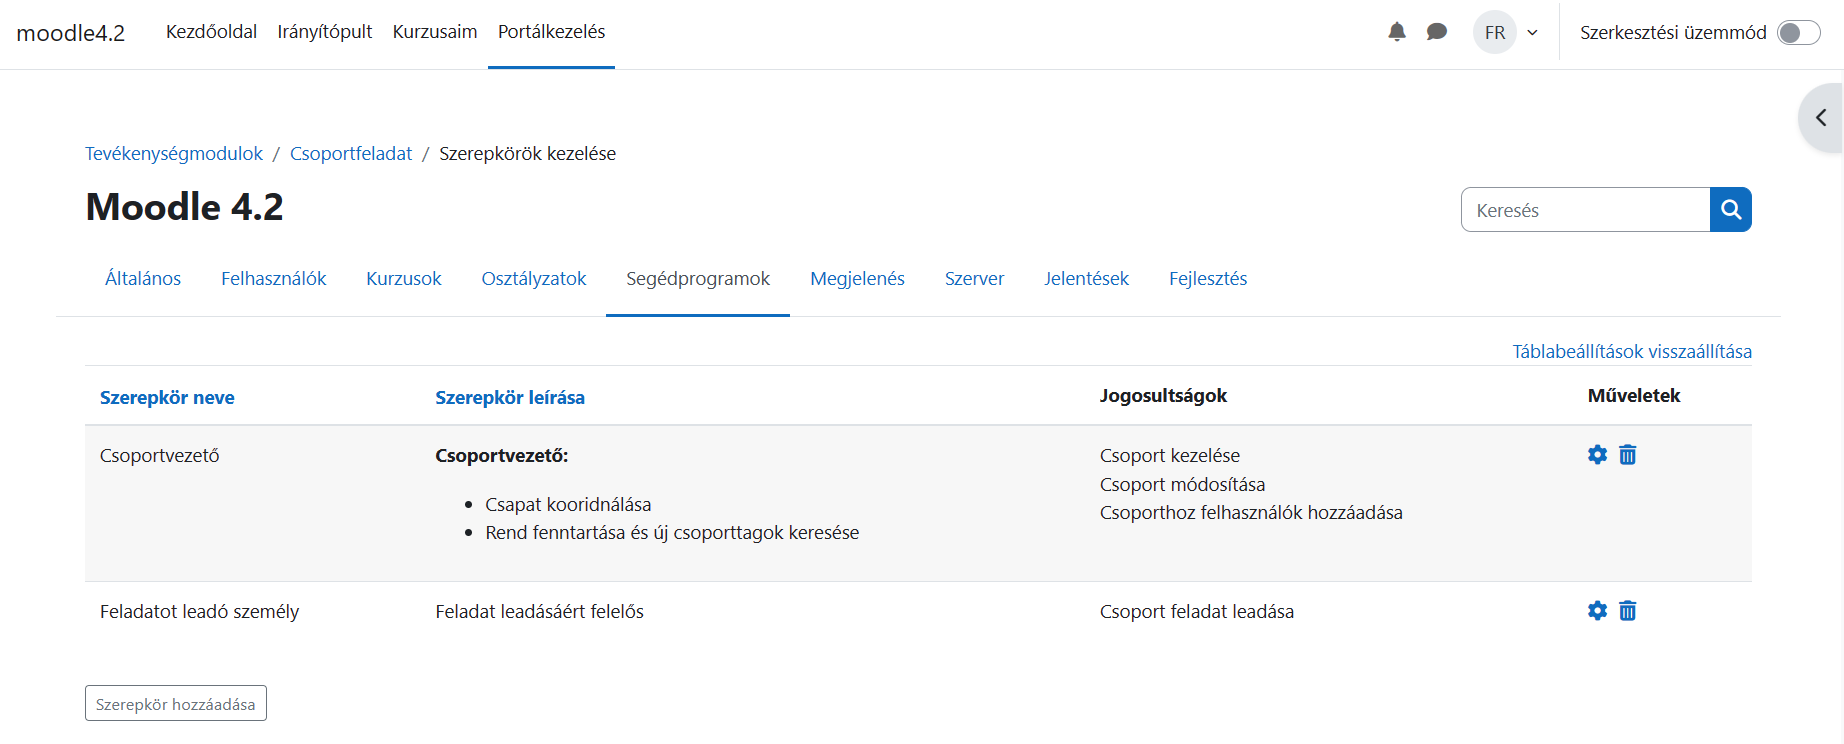
\includegraphics[width=0.8\textwidth,frame]{images/szerepkorok_kezelese.png}
	\caption{Szerepkörök áttekintése}
\end{figure}

\subsection{Szerepkör létrehozása, módosítása és törlése  }

A szerepkörök kezelése menüpontból érhető el az új szerepkör létrehozása opció. Meglévő szerepkör esetén a fogaskerék ikonra kattintva a szerepkör adatait módosíthatjuk. A kuka ikonra kattintás után egy biztonsági ellenőrzés után a szerepkör törlésre kerül. A szerepkör létrehozási és módosítási menüpontban a szerepkör nevét, leírását és jogosultságait adhatjuk meg. A szerepkörnek az elérhető jogosultságok közül akármennyit megadhatunk. Ezek a jogosultságok a tanulóknak csak a csoportjukon belül lesznek elérhetőek. Fontos, hogy a szerepkörünk törlésével a csoportban keletkezett összes felhasználó szerepkör hozzárendelés törlődik, így a törölt szerepkörrel rendelkező csoporttagok innentől szerepkör nélküli tagként fognak viselkedni..

\begin{figure}[H]
	\centering
	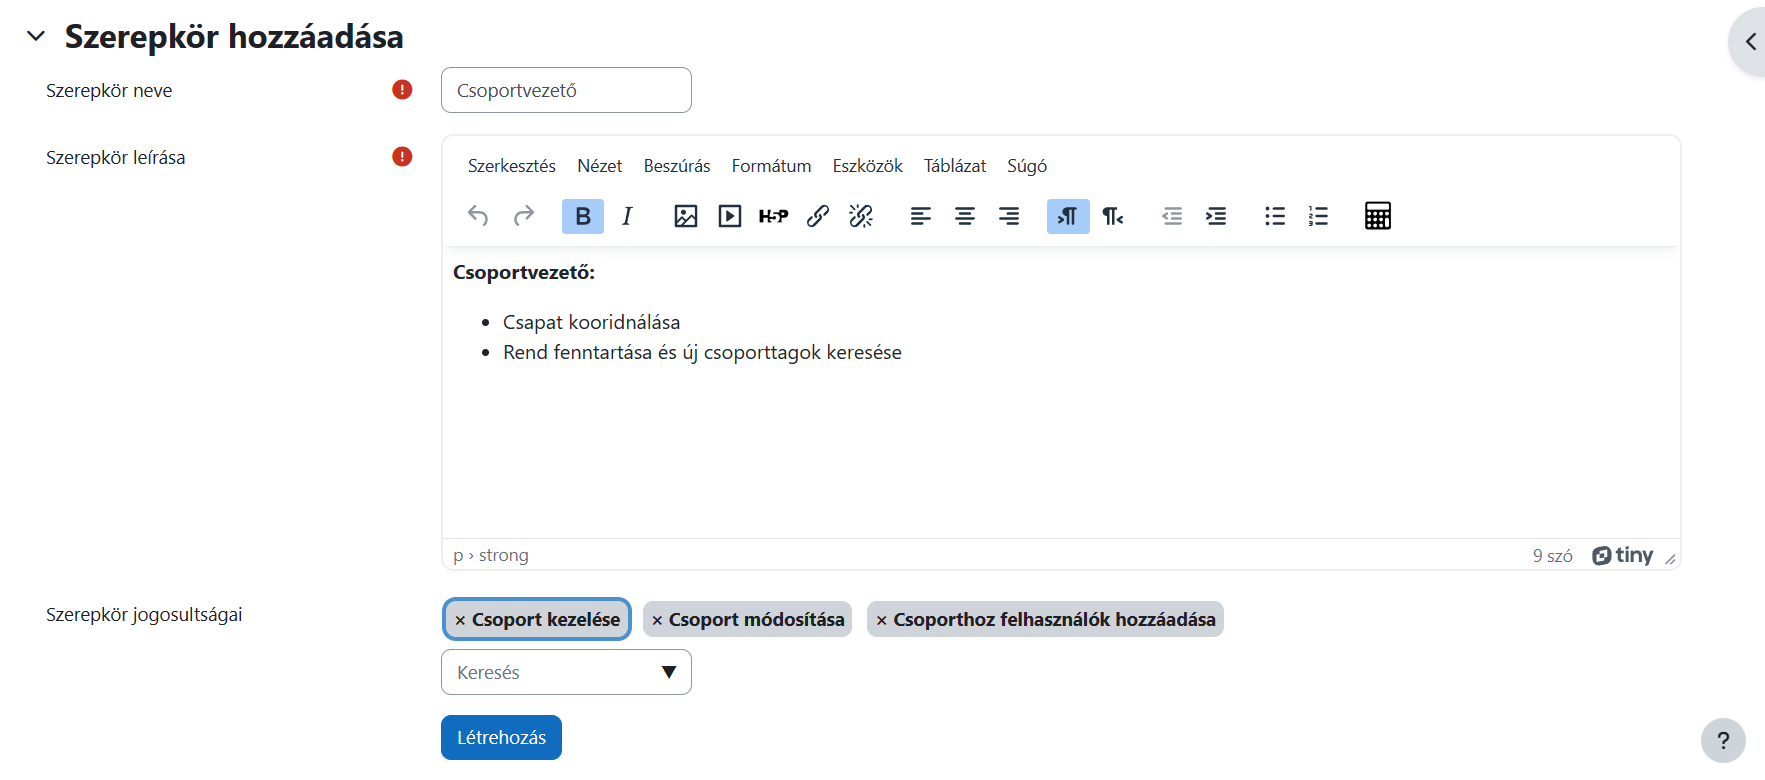
\includegraphics[width=0.8\textwidth,frame]{images/szerepkor_letrehozas.png}
	\caption{Szerepkör létrehozása űrlap}
\end{figure}

\section{Tanárok funkciói}

A segédprogram a tanárok számára adja a legtöbb lehetőséget funkcionalitás terén. A tanárok a kurzuson belüli összes beállítási és konfigurációs felületet elérik, emellett a tevékenységen belül is csoport és feladatszervezési beállításokat tudnak módosítani. Tanárnak az számít, aki a kurzus vagy a tevékenység kontextusában\footnote{Kontextus: Környezet, a Moodle-ben minden oldal rendelekzik egy kontextussal, amin belül többletjogokat adhatunk felhasználóknak.} rendelkezik a \textit{teacher} vagy az \textit{editingteacher} szerepkörrel.

\subsection{Tevékenységmodul kezelése}

Tanárként tudunk a kurzuson belül új tevékenységeket hozzáadni. Itt van lehetőségünk egy új modul típus, a Csoportfeladat kiválasztására. A modul általános beállításain kívül van lehetőségünk pontozási rendszert beállítani a tevékenységünknek. A pontozási rendszer a Moodle által támogatott Skála és Pont alapján történhet. Teljesítési beállításoknál elérhetőek a következő opciók:

\begin{compactitem}
    	\item Tevékenység megtekintése: a felhasználónak elég megnyitni a modult, a teljesítési feltétel a megnyitás pillanatában teljesül.
        \item Osztályzat megszerzése: a felhasználónak szükséges osztályzatot szerezni a teljesítéshez. Az osztályzat eredménye itt nem számít. Érdemes Skála alapú pontozásnál alkalmazni.
        \item Megfelelt osztályzat megszerzése: a felhasználónak szükséges osztályzatot szerezni a teljesítéshez. Az osztályzat eredménye ha alacsonyabb, mint a teljesítéshez megadott pontszám, a felhasználó nem teljesíti a modult. Érdemes Pont alapú pontozásnál alkalmazni.
\end{compactitem}

Ha szeretnénk a kurzus teljesítését értékeléshez kötni, a modulunk minden esetben létrehoz egy pontozási tételt, így a kurzus pontozási riportjában is látható lesz mint új oszlop. A pontozási menün belül, a beadási határidőt is megszabhatjuk, így tudjuk jelezni a hallgatók felé a feladat véghatáridejét.

A tevékenység létrehozása után a modul elérhető lesz a kurzuson belül és lehetőségünk lesz a csoportok létrehozására.

\begin{figure}[H]
	\centering
	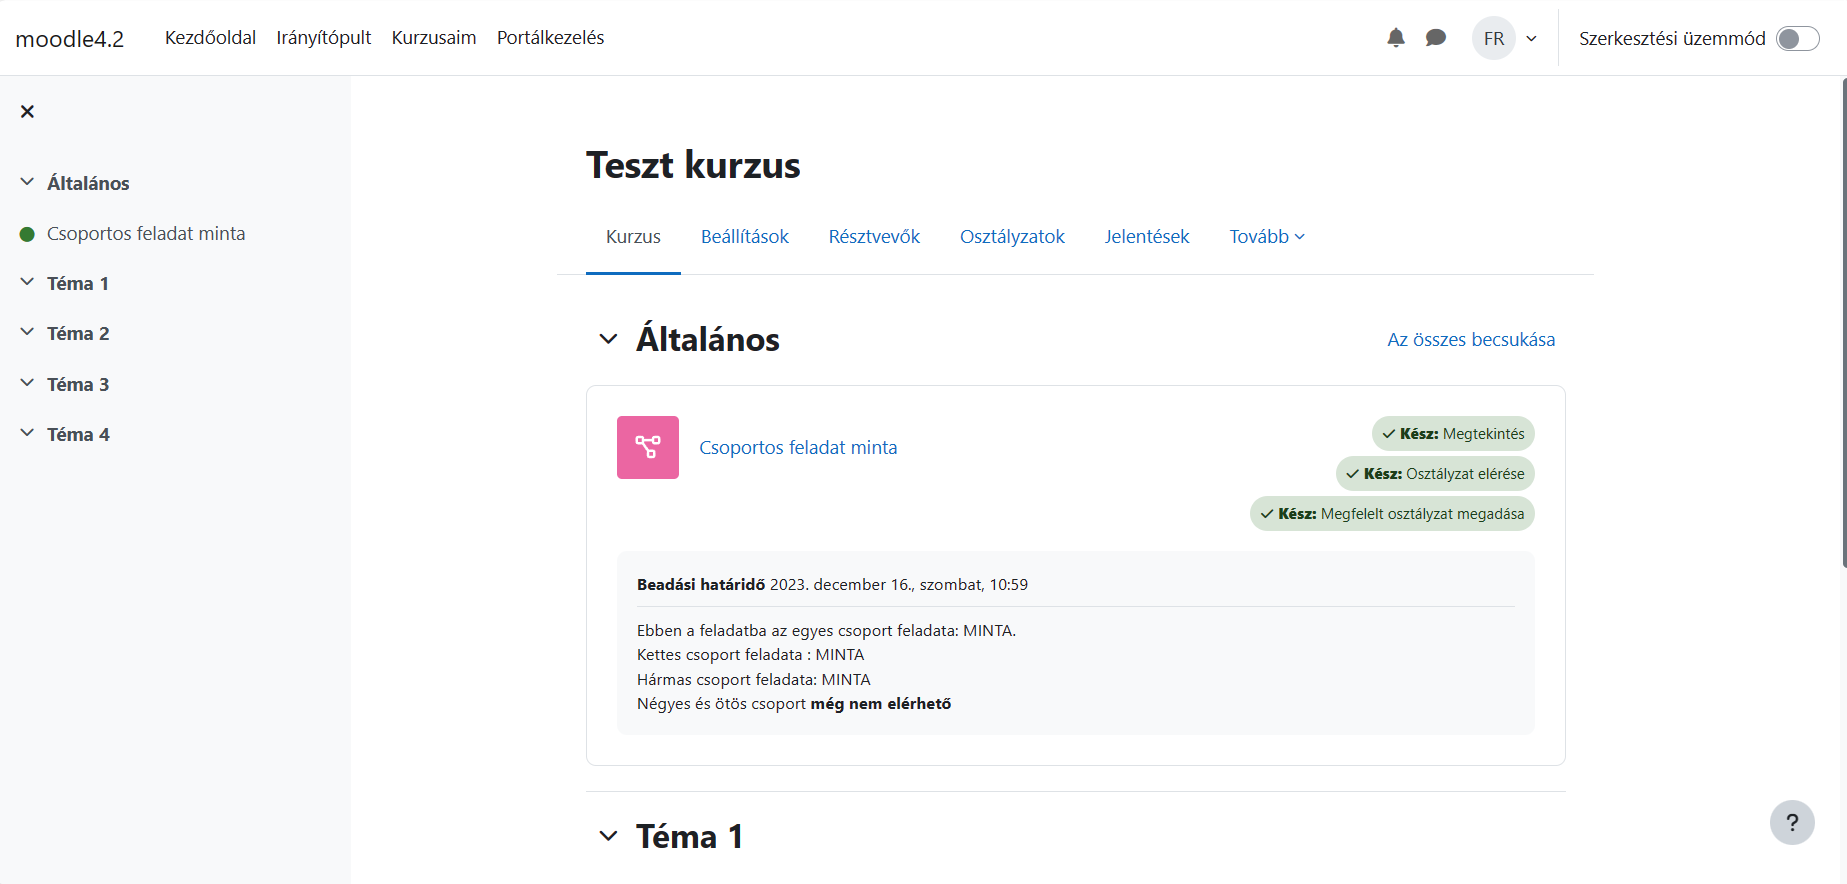
\includegraphics[width=0.8\textwidth,frame]{images/tevekenyseg_nezet.png}
	\caption{Új Csoportfeladat tevékenységmodul a kurzusunkban}
\end{figure}

Mivel a Csoportfeladat támogatja a Moodle Backup funkcióit, így lehetőségünk van a kurzus felületen duplikálni az ilyen típusú kurzusmodulokat. Duplikálásnál felhasználói adatok nem kerülnek át az új tevékenységbe, csak a csoportok és a tevékenység beállításai.

\subsection{Engedélyek kezelése}

Az alkalmazásban a következő egyedi jogosultságok érhetőek el:
\begin{compactitem}
    	\item Csoportmegjegyzés írása: a felhasználó megjegyzést írhat a csoportja csevegésébe. Fontos előfeltétele a jogosultságnak, hogy a felhasználónak rendelkeznie kell csoporttal.
     \item Csoport létrehozása: új csoport létrehozása.
     \item Csoport kezelése: meglévő csoport adatainak módosítása. Hallgatók esetén ez a jogosultság csak saját csoport módosítására ad lehetőséget, ha szerepkörön keresztül került hozzáadásra a jogosultság.
     \item Csoport törlése: meglévő csoport és azzal kapcsolatos összes adat törlése.
     \item Csoporthoz felhasználók hozzáadása: új csoporttagok felvétele a csoportba. Hallgatók esetén ez a jogosultság csak saját csoport módosítására ad lehetőséget, ha szerepkörön keresztül került hozzáadásra a jogosultság.
     \item Csoport értékelése: csoportok értékelése felület elérhetőségét korlátozza.
     \item Csoport feladat leadása: a felhasználó csoportjának leadási felületének elérhetőségét tudjuk vele korlátozni. 
\end{compactitem}

\begin{figure}[H]
	\centering
	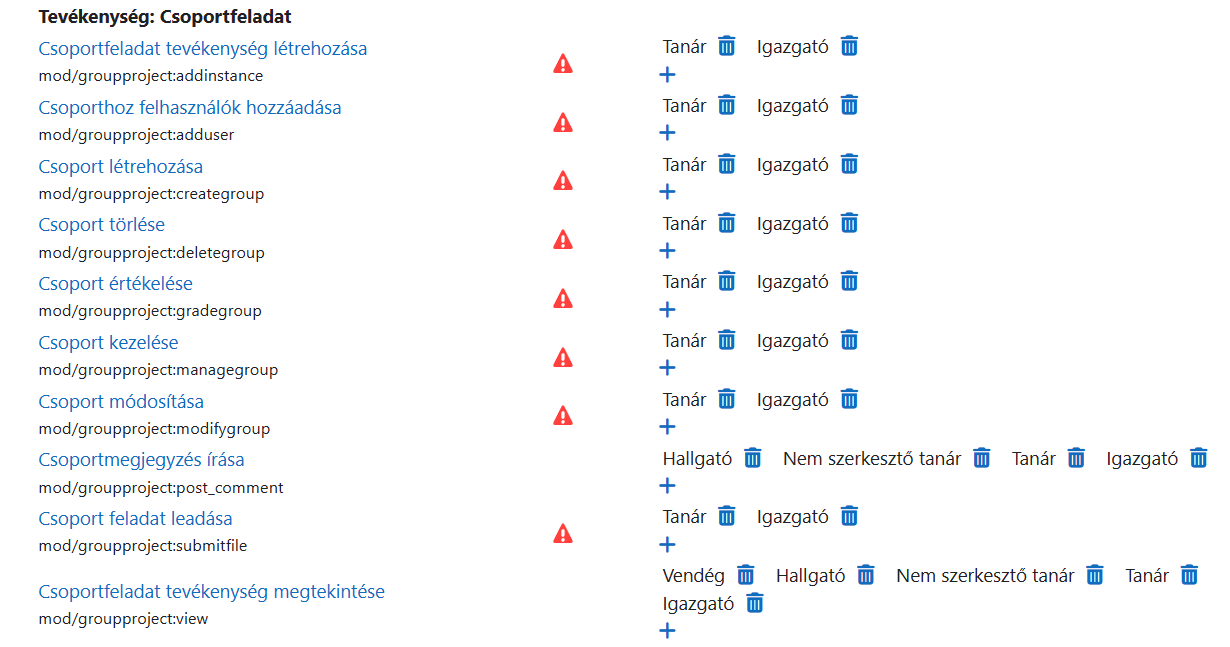
\includegraphics[width=0.8\textwidth,frame]{images/engedelyek.png}
	\caption{Elérhető engedélyek a modulban}
\end{figure}

A jogosultságok, mind tevékenység szinten kerültek definiálásra, így egyedileg módosíthatóak akár kurzuson belül is, ha van két tevékenységünk.

\subsection{Csoportok kezelése}

Ha a tevékenységre kattintunk a tanárok a \textit{Csoportok kezelése }oldalra irányítódnak át. A csoport kezelési felületen a tanárok egy összegző felületet látnak, ahol az eddig létrehozott csoportok találhatóak. Itt tudunk új csoportot létrehozni, meglévőt módosítani vagy akár törölni. A táblázat tartalmazza a csoport nevét, a csoport jelenlegi és maximális létszámát. A csoport által beadott munka is letölthető az oldalról, illetve a csoport által szerzett értékelés is megjelenik a táblázatban. A tanárok megtekinthetik az elérhető szerepköröket (egy linken keresztül), viszont módosítani nem módosíthatják azokat.

\begin{figure}[H]
	\centering
	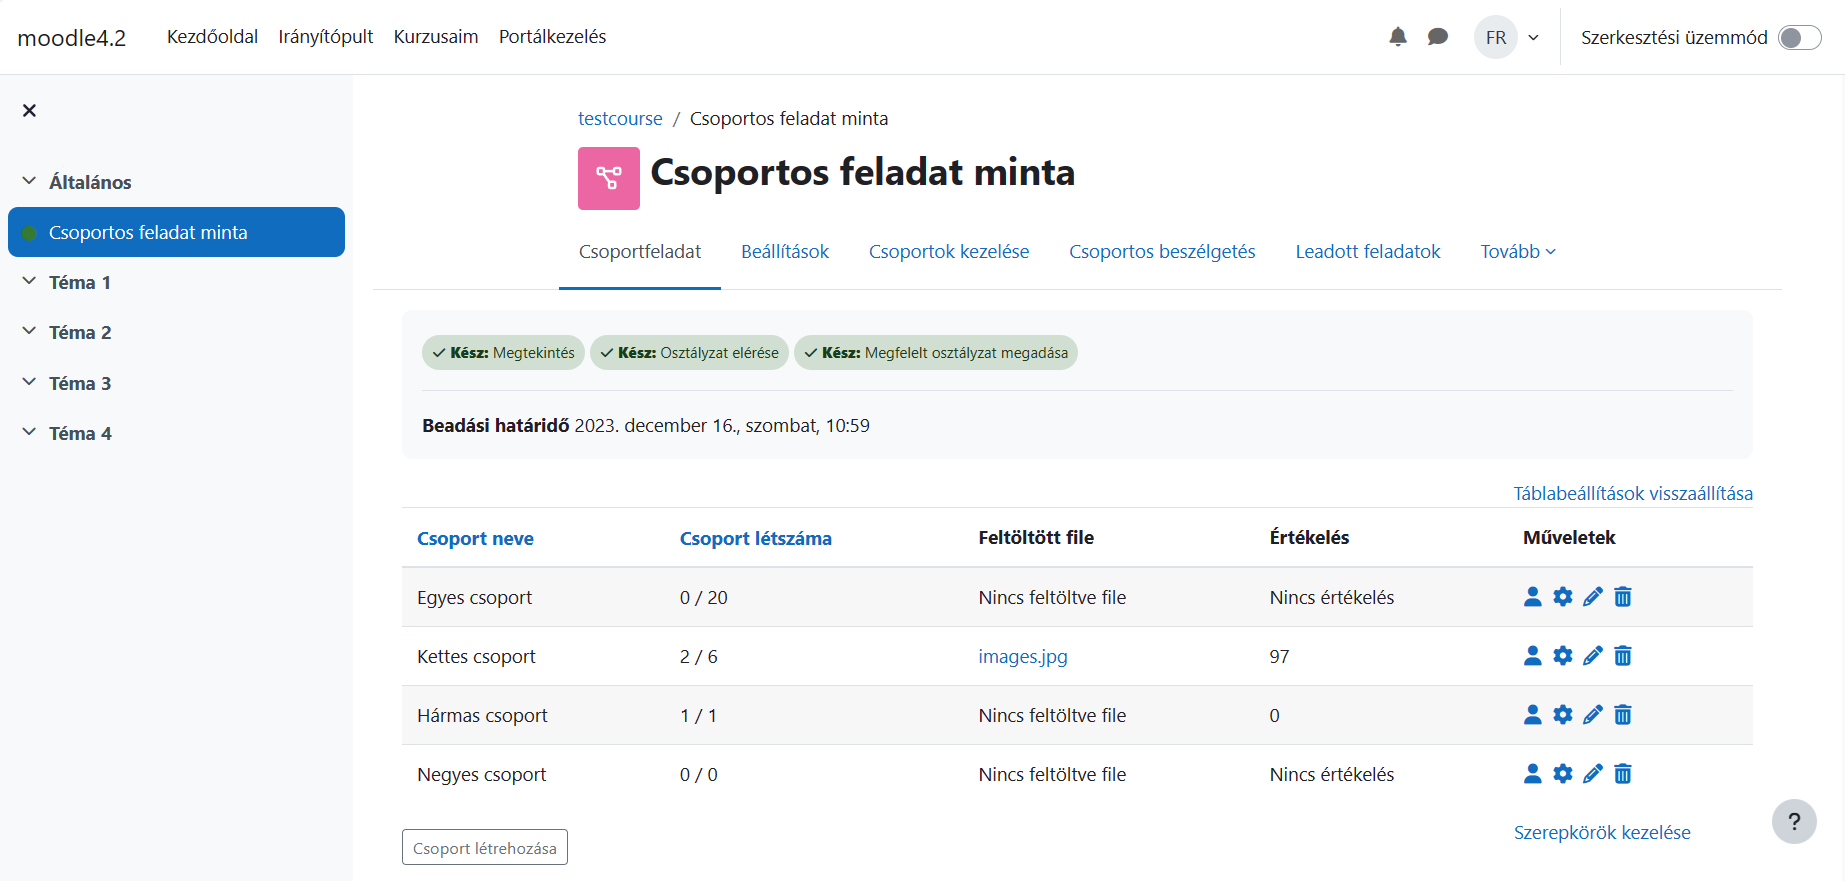
\includegraphics[width=0.8\textwidth,frame]{images/csoportok_kezelese.png}
	\caption{Csoportok kezelése tevékenységmodulban}
\end{figure}

\subsection{Csoport létrehozása, módosítása és törlése}

A csoportok kezelése menüpontból érhető el az új csoport létrehozása opció. Meglévő csoport esetén a fogaskerék ikonra kattintva a csoport adatait módosíthatjuk. A kuka ikonra kattintás után egy biztonsági ellenőrzés után a csoport törlésre kerül. A csoport létrehozási és módosítási menüpontban a csoport nevét, azonosítóját és létszámát adhatjuk meg. A csoportlétszám korlátozni fogja az egyszerre aktív csoporttagok számát. Fontos, hogy a csoportunk törlésével a csoportban keletkezett összes adat törlődik, így a csoport tagjainak üzenetei, fájljai, értékelései mind törlődnek a csoporttal együtt.

\begin{figure}[H]
	\centering
	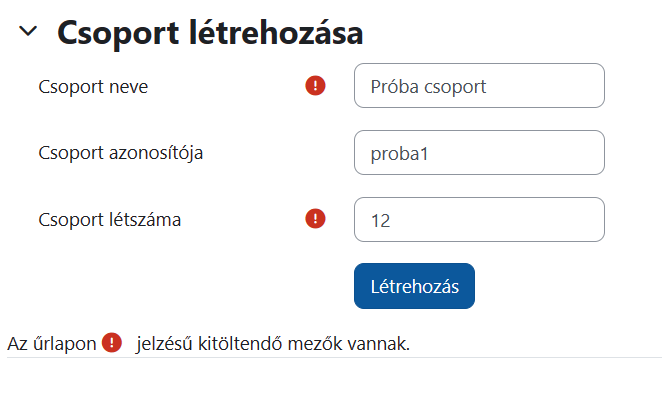
\includegraphics[width=0.8\textwidth,frame]{images/csoport_letrehozas.png}
	\caption{Csoport létrehozása űrlap}
\end{figure}

\subsection{Csoporttagok felvétele}

A csoportok kezelése menüpontból elérhető a csoporttagok felvételi oldala. Meglévő csoport esetén a Műveletek oszlopban található ember ikonra kattintással érhetjük el az oldalt. Ha a csoport nem üres, akkor a meglévő csoporttagok listáját fogjuk látni, a hozzájuk rendelt szerepkörökkel. A csoporttag neve és szerepköre mellett egy kuka ikon is található, amivel ki tudjuk törölni a felhasználót a csoportból. A potenciális felhasználók listáját a segédprogram a kurzusba beíratott felhasználók közül válogatja ki. Olyan felhasználók akik már másik csoport tagjai nem fognak megjelenni a potenciális felhasználók között. Új felhasználó felvételére egészen addig van lehetőségünk még a csoportlétszám be nem telik. Új csoporttagot akár szerepkör nélkül is fel tudunk venni. Az űrlap csak akkor kerül mentésre ha leadjuk azt a Felhasználók hozzáadása gombbal. A törölt felhasználók üzenetei megmaradnak a csoportban, egyéb adatai elvesznek.

\begin{figure}[H]
	\centering
	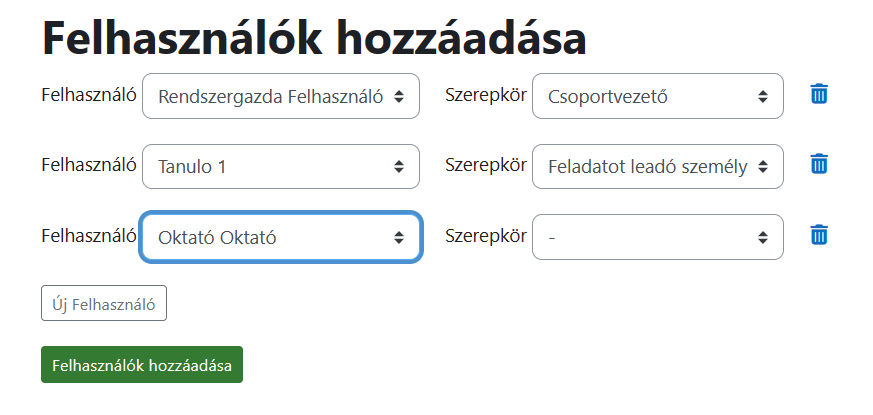
\includegraphics[width=0.8\textwidth,frame]{images/felhasznalok_hozzaadasa.png}
	\caption{Felhasználók hozzáadása űrlap}
\end{figure}

\subsection{Csoportok értékelése}

A modul lehetőséget ad a Moodle által támogatott összes pontozási lehetőségre. A tevékenység létrehozásakor megadott pontozási módszerrel (ha beállításra került) képes a pontozást végző tanár értékelést adni a csoportnak. Ezen módszerek lehetnek Pont, illetve Skála alapúak. Ha pontozás megtörtént, az értékelés a csoportban lévő összes hallgató számára beírásra kerül. A kurzus összegző felületén, az összegző riportban jelenik meg a hallgatók összpontszáma, a modulban kiosztott pontszámok alapján. Az értékelés a csoport összegző felültén is meg fog jelenni.

\begin{figure}[H]
	\centering
	\subcaptionbox{Pontszám alapú eredmény megadása}{
		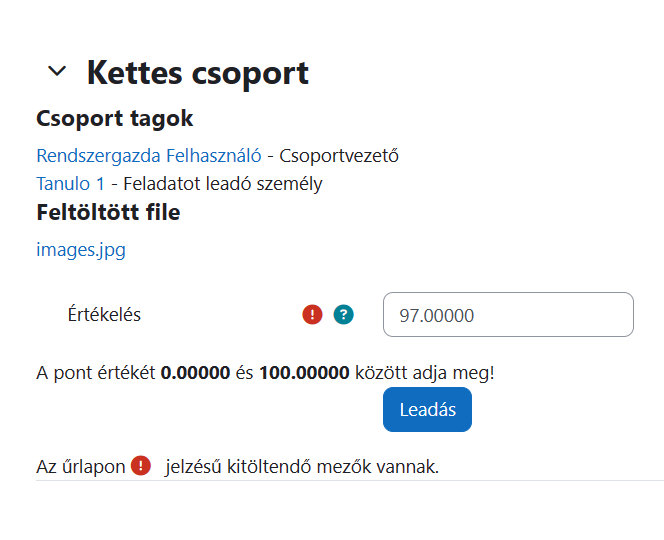
\includegraphics[width=0.45\linewidth,frame]{images/pontszam_pontozas.png}}
	\hspace{5pt}
	\subcaptionbox{Skála alapú pontszám megadása}{
		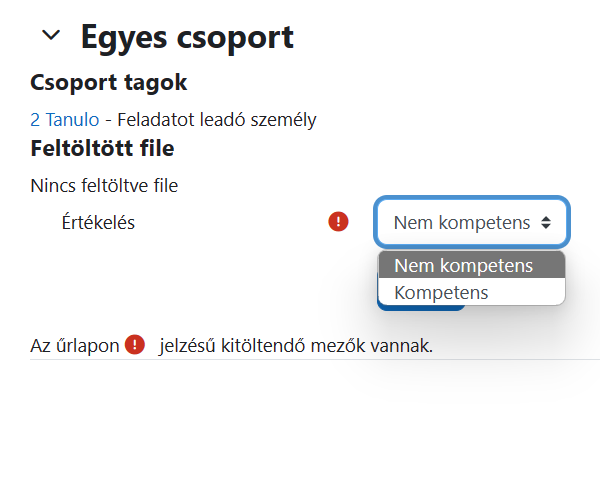
\includegraphics[width=0.45\linewidth,frame]{images/skala_pontozas.png}}
	\caption{Pont és skála alapú értékelés összehasonlítása}
	\label{fig:example-2}
\end{figure}

\subsection{Biztonsági mentés, visszaállítás és importálás funkció}

A Moodle által támogatott \textit{Backup} funkció is támogatott a segédprogramon belül. Tanárként tudunk biztonsági mentést készíteni a tevékenységmodulunk jelenlegi állapotáról. Ezt a biztonsági mentést tárolni fogja a Moodle és lehetőségünk lesz visszaállítani a modult egy régebbi állapotra. A biztonsági mentés nem csak abba a rendszerbe tölthető vissza, ahol a mentés megtörtént. A segédprogramunk által generált adatokat tetszőleges Moodle rendszerbe tudjuk visszatölteni. (persze csak abban az esetben, ha a másik rendszer is rendelkezik a segédprogramunkkal). Az importálás funkció a fent említett két művelet egy időben való végrehajtása: készül egy biztonsági mentés a modulunk állapotáról, majd ezt a biztonsági mentést visszatöltjük egy meglévő vagy új kurzusba. A mentés és importálás során el tudjuk dönteni, hogy a felhasználói adatokat is szeretnénk-e átvinni az új modulba. Fontos, hogy ha ezzel a lehetőséggel nem élünk, akkor a felhasználói csoporthozzárendelések, leadott fájlok, csoportok jegyei illetve a csoportok beszélgetései nem kerülnek migrálásra. 

\section{Hallgatók funkciói}

A hallgatók igazán csak akkor tudják az applikáció adta lehetőségeket kihasználni ha egy csoport tagjai lesznek. A csoporton belül minden hallgatónak lehet egy egyedi szerepe, amit a csoporttagság kezdetekor kapott. Ezekkel a szerepekkel egyes csoporttagoknak többletjogot adhatunk.

\subsection{Csoportos csevegés}

Ha a hallgató egy csoport tagja, a tevékenységre kattintás után rögtön a csoportos beszélgetés menübe kerül, ahol látja az éppen aktív csoportjának csevegését. A beszélgetés szinkron módon történik, így a hallgatók valós időben tudják egymással megosztani a feladat részleteit, illetve a megoldás közben felmerülő problémákat. (A leadott változatában a programban beállításra került egy 8 másodperces késleltetés prezentációs célokból) A csoporttagok profilképei is megjelennek a beszélgetés közben, amire ha a hallgató rákattint, a felhasználó profiloldalára irányítódik át. A beszélgetés üzenetküldésére egy TinyMCE\footnote{TinyMCE: WYSIWYG HTML szerkesztő, \url{https://www.tiny.cloud/tinymce/}} multifunkcionális szerkesztő áll rendelkezésre, mely képes képek, emoji-k, és HTML tartalmak értelemezésére, így az üzenet tartalma lényegében bármi lehet. A beszélgetésben való részvétel is egy jogosultsághoz van kötve, viszont ezzel minden hallgató rendelkezik. A portáladminisztrátorok képesek ezt a jogosultságot elvenni a felhasználótól, ha nem megfelelően kommunikál tanulótársaival.
\begin{figure}[H]
	\centering
	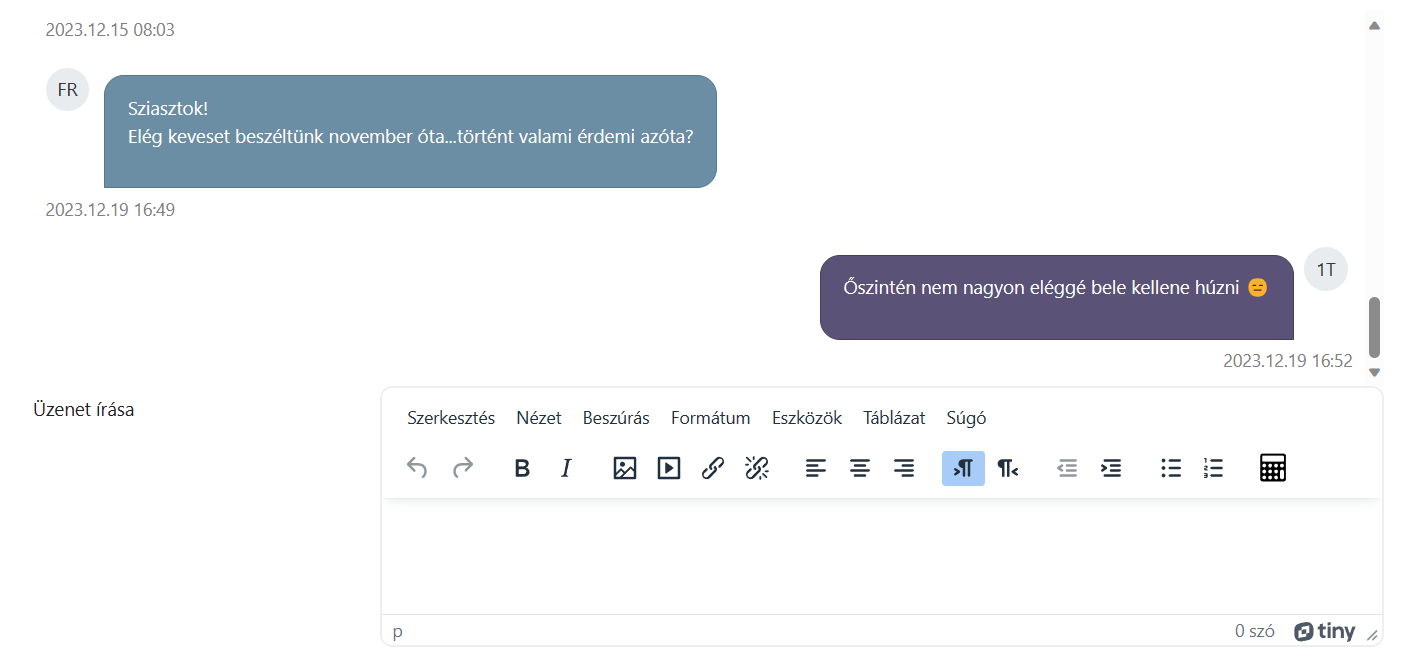
\includegraphics[width=0.8\textwidth, frame]{images/uzenet.png}
	\caption{Beszélgetés a csoporton belül}
\end{figure}

\subsection{Feladat leadása}

Ha a csoport elkészült a feladatával, lehetősége van az arra kijelölt személynek feltölteni a megoldást a \textit{Leadott feladatok} menüpontban. Egy feladatot többször is le lehet adnia a csoportnak, de mindig a legfrissebb leadás fog megjelenni az értékelő tanároknak. A feladat leadására a Moodle fájlkezelője áll rendelkezésre, így már a portálra korábban feltöltött fájlok között is tudnak a felhasználók böngészni. A feladat feltöltési korláta a rendszerben és PHP-ban beállított feltöltési korlátnak felel meg. A hallgatónak csak egy fájlfeltöltésre van lehetősége, viszont az állomány típusa nem számít, így tömörített állományt is elfogad az alkalmazás. Feladatot egészen a beadási határidőig tölthet fel a csapat, ez a határidő minden menüpontban megjelenik a hallgatók számára a modulon belül. A leadott feladatok biztonsági mentésnél is elmentésre kerülnek.
\begin{figure}[H]
	\centering
	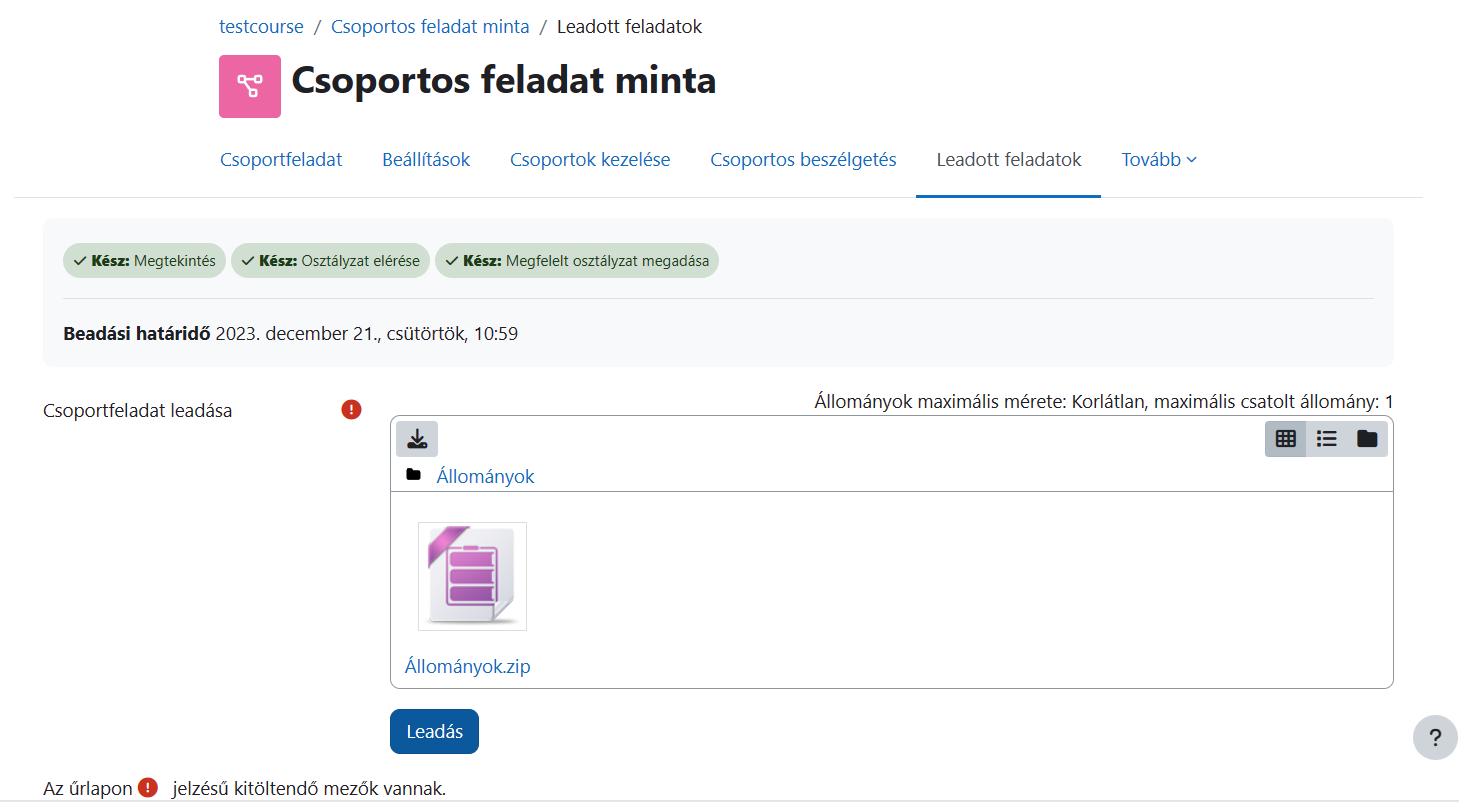
\includegraphics[width=0.8\textwidth, frame]{images/feladat.png}
	\caption{Feladat leadási felület}
\end{figure}

\subsection{Egyéb oldalak}

A hallgatóknak lehetőségük van bizonyos oldalak korlátozott elérésére. Ha megfelelő szerepkörrel rendelkeznek a csoporton belül, akkor van lehetőségük új csoport létrehozására. Saját csoportjuk adatainak módosítására is kaphatnak jogosultságot, így tudják növelni manuálisan a csoportlétszámot, ha több tagra van szükségük. Emellett van lehetőségünk saját csoportjukhoz új tagokat felvenni a navigációs menün keresztül. A feladat leadása is szerepkör jogosultsághoz kötött. Ha szeretnénk, hogy minden csoporttag leadhassa a feladatot, akkor az \textit{Engedélyek} menüponton keresztül hozzá kell adnunk a Hallgatót a \textit{Csoport feladat leadása} engedélyhez. A felhasználó jogosultságától függően a modul navigációs sávjában megjelenhetnek új menüpontok, amik a felhasználót az általa elérhető oldalra navigál tovább. Ha a felhasználó olyan oldalt szeretne elérni, amihez nem rendelkezik a szükséges jogosultsággal, akkor egy általános hibaüzenetet (Jogosultság megtagadva) kap a felületen.

\begin{figure}[H]
	\centering
	\subcaptionbox{Navigációs menü jogosultság nélkül}{
		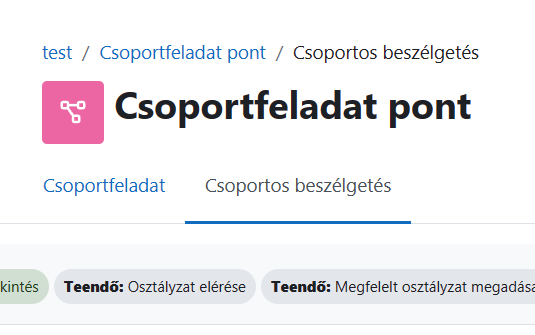
\includegraphics[width=0.35\linewidth,frame]{images/navigacio_ures.png}}
	\hspace{5pt}
	\subcaptionbox{Navigációs menü az összes jogosultsággal}{
		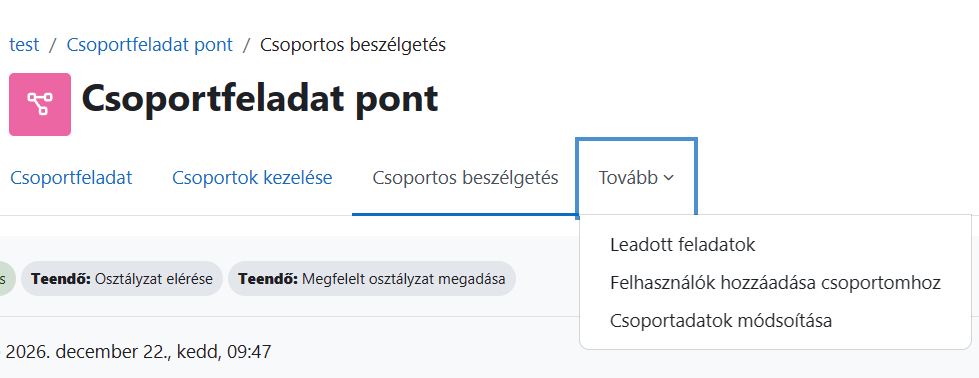
\includegraphics[width=0.55\linewidth,frame]{images/navigacio_teljes.png}}
	\caption{Navigációs menü dinamikus megjelenése}
	\label{fig:example-2}
\end{figure}